\section{Neutrino Physics Historical Overview}
\label{Chapter:1}

\subsection{The Beta Decay Problem}

Radioactivity was discovered in 1896 by Henri Becquerel. A few years later, in 1899, Ernest Rutherford classified radioactivity emissions into two types: $\alpha$ and $\beta$. In the occasion, Rutherford conjectured that the beta decay was a two-body decay. In such case, the decay would be characterized by a nucleus A becoming a lighter nucleus B, with the emission of an electron, like the following:
%
\begin{equation}
	A \longrightarrow B + e^- .
\end{equation}
%
Consequently, the energies of the outgoing particles would be kinematically determined. 
Using conservation of energy and momentum, it is straightforward to conclude that this energy should be:
%
\begin{equation}
	E = \frac{m_A^2 - m_B^2 + m_e^2}{2m_A} c^2.
	\label{electron_max_energy} 
\end{equation}
%
Experiments conducted by Lise Meitner and Otto Han in 1911 demonstrated that the energy spectrum of the electron coming out of the $\beta$ decay was, in fact, not well-defined, as expected if it was two-body decay. The electron energy spectrum was continuous, having the maximum energy defined by the equation \ref{electron_max_energy} (see figure \ref{figure_the_beta_decay_spectrum_of_tritium}) \cite{griffiths}.
%
\begin{figure}[h!]
	\begin{center}
		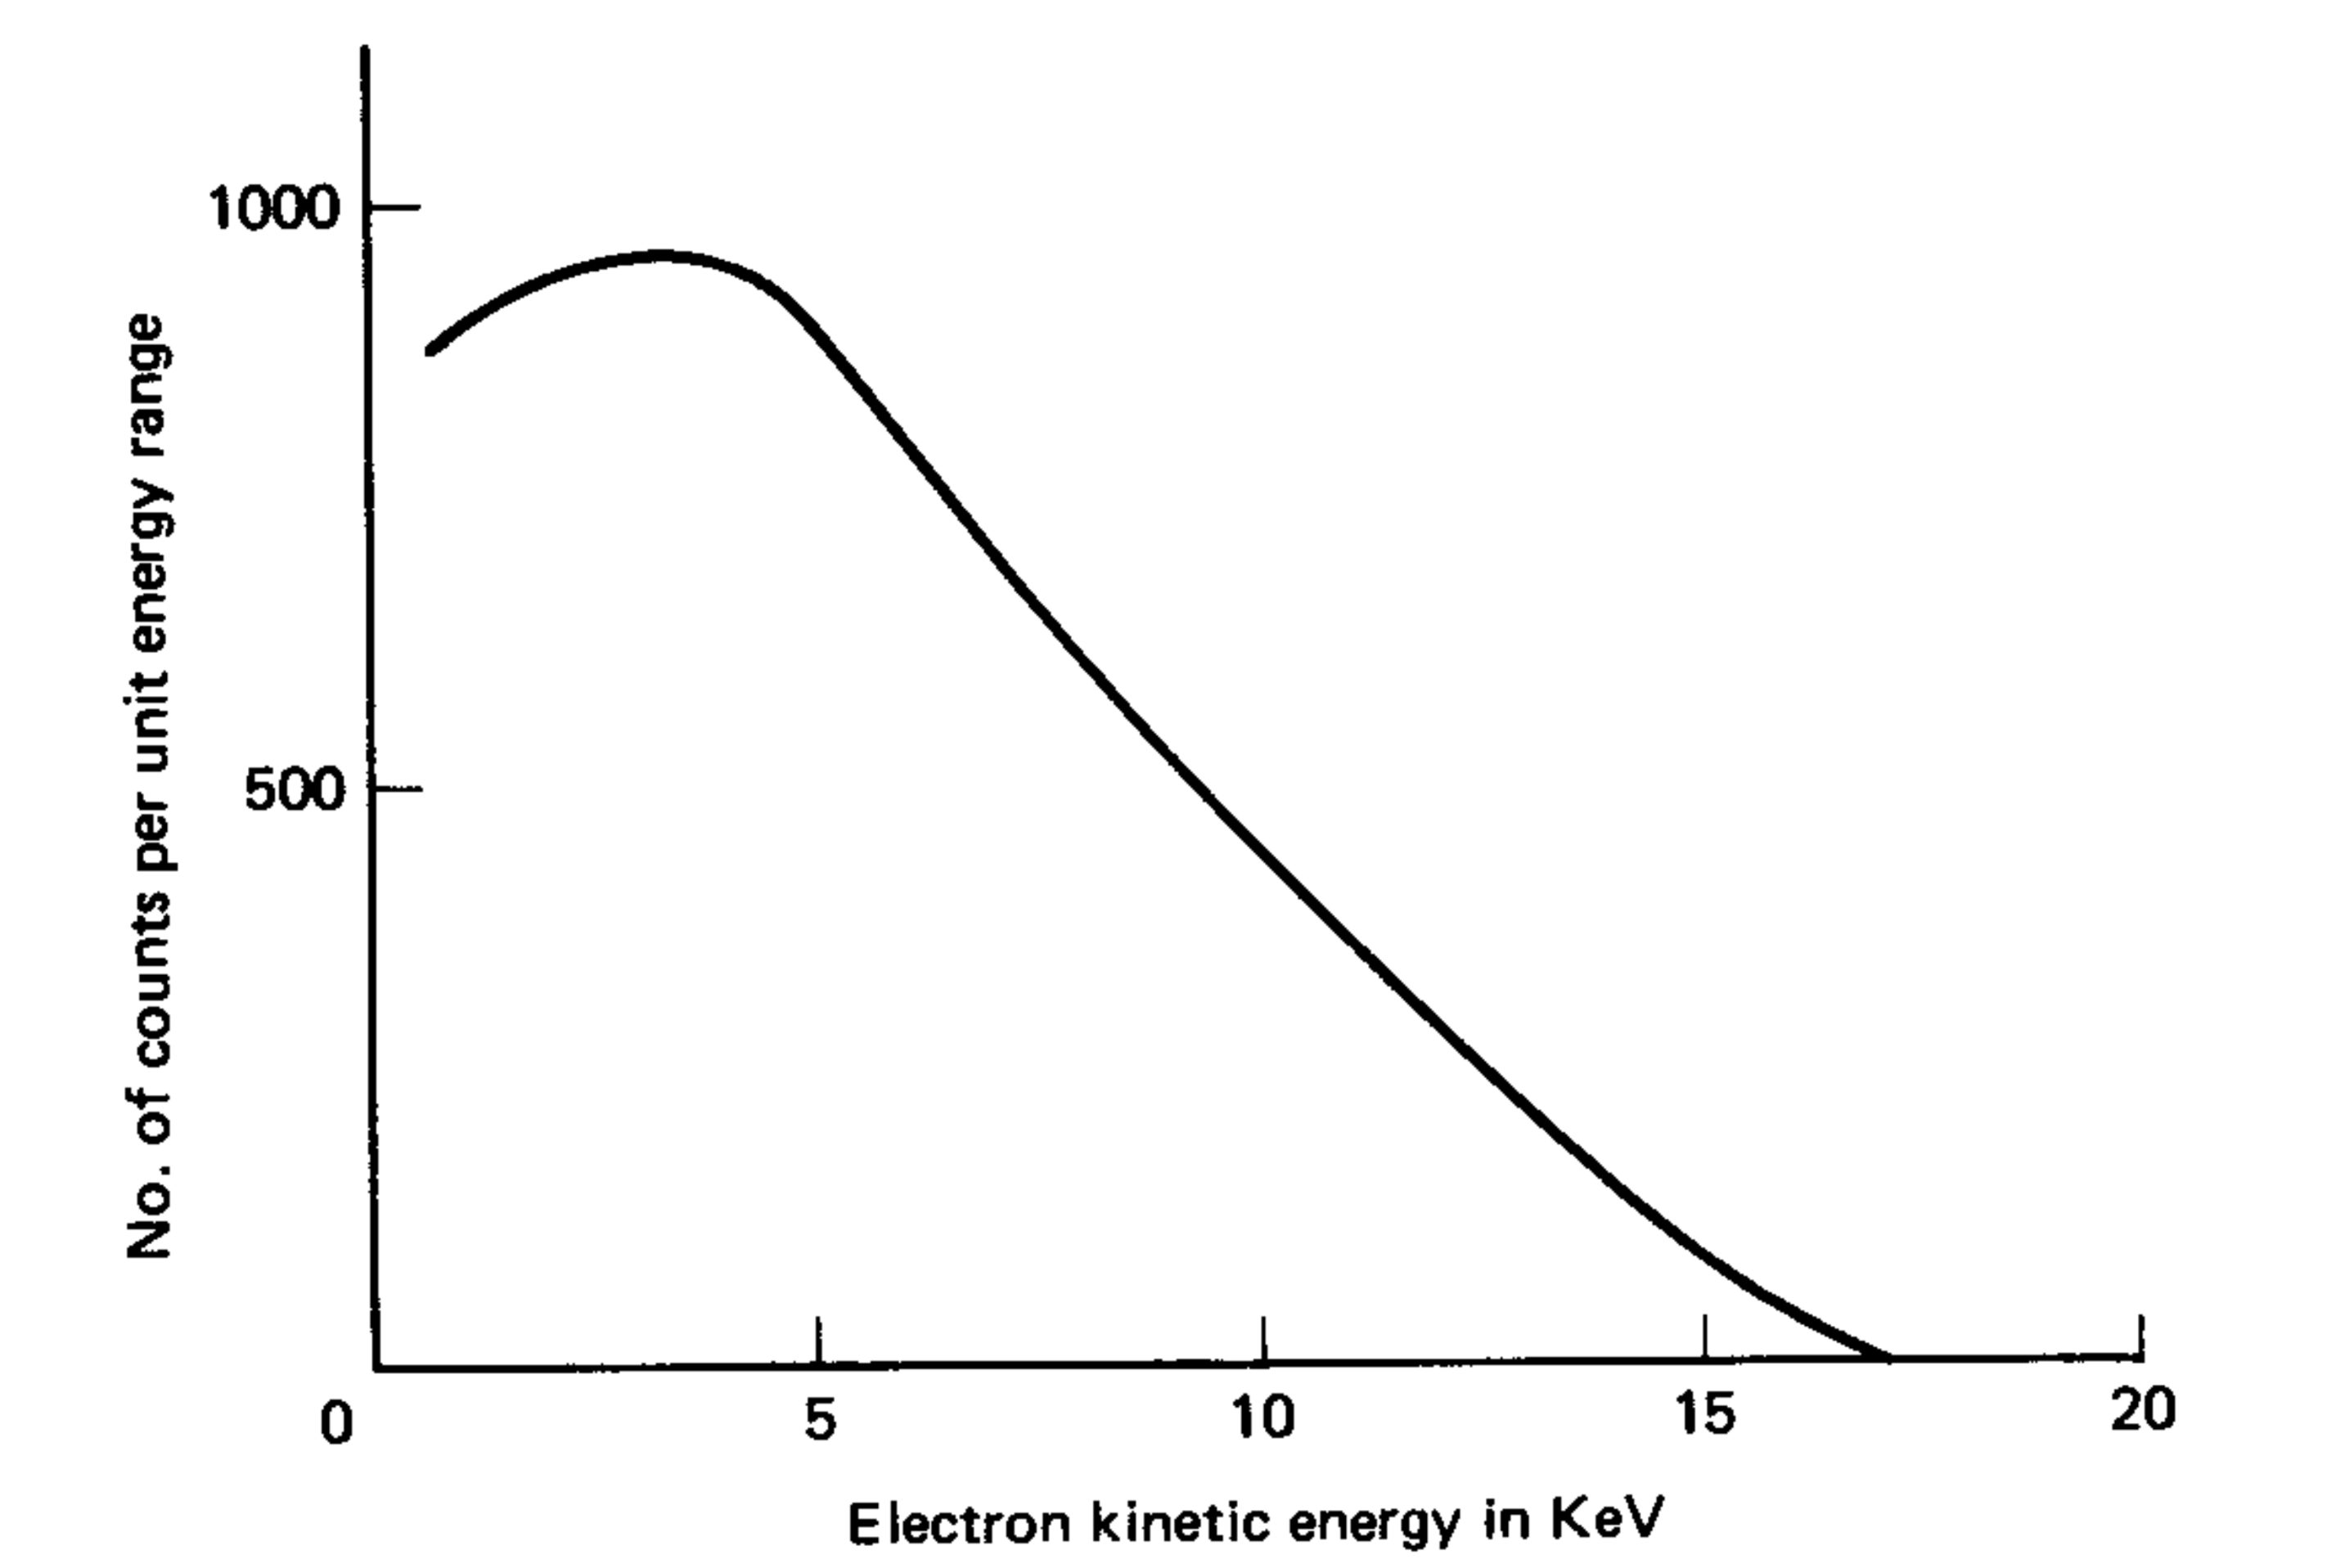
\includegraphics[scale=0.3]{Figures/electron_beta_decay_spectrum.pdf}
		\caption[The beta decay spectrum of tritium]{ {\textbf{The beta decay spectrum of tritium}} \\The figure shows the electron energy spectrum in a beta decay of tritium \cite{griffiths}.}
		\label{figure_the_beta_decay_spectrum_of_tritium}	
	\end{center}
\end{figure}
%

In 1930, Wolfgang Pauli proposed that the beta decay was not a two-body decay, but a three-body decay. He predicted that the third particle proposed by him would be neutral and light. Pauli originally named it neutron. Later, with Chadwick's discovery of the neutron, Fermi changed the name of his predicted particle to neutrino \cite{griffiths}. A few years later, in 1933, Pauli and Perrin proposed that neutrinos were massless \cite{griffiths}.

\subsection{The First Neutrino Measurement}
It was not until 1956 that neutrinos were experimentally verified by Cowan and Reines. They conducted an experiment at the Savannah River nuclear reactor in South Carolina that consisted of a big tank of water and cadmium chloride, surrounded by 4,200 litters of liquid scintillator, seated near the nuclear reactor. If neutrinos, as predicted by Pauli, were real, they would be produced by the nuclear reaction inside the reactor and, as entering the detector, would possibly hit the protons of the water and produce a positron and a neutron. This reaction is called inverse beta decay, and it is given as:
%
\begin{equation}
	\overline{\nu} + p^+ \longrightarrow n + e^+.
	\label{inverse_beta_decay_eq}
\end{equation}
%
The reaction's signature they were looking for were two photons, produced by the electron-positron annihilation, and, a few microseconds later, a few photons, produced by the neutron capture by the cadmium \cite{nobel_leptons}. They published their results in a paper called “Detection of the Free Neutrino: A Confirmation”, confirming the existence of neutrinos (Ref. \cite{cowan_reines}). 


\section{Different Types of Neutrinos}
In 1953, Konopinski  and Mahmoud proposed the existence of a lepton number and the conversation of it, which could explain why certain reactions happen and some others do not. As convention, it was established that leptons would have a lepton number L = 1, that antileptons would have lepton number L = $-$1, and that any other particle would have lepton number L = 0. By this rule, an antineutrino should be produced in a beta decay. Although the rule explained why many reactions supposedly allowed to happen were not observed, it still did not explain a few cases. This led them to postulate the existence of a lepton number for each of the leptons. That is, a muon number, an electron number and, years later, a tau number (see table \ref{lepton_family}) \cite{Konopinski_Mahmoud}. 
%
\begin{table}
	\begin{center}
		\begin{tabular}{cccc}
			\bottomrule
						& \textbf{Lepton number}	&	\textbf{Electron number}	&	\textbf{Muon number}\\
			\toprule
			Leptons			&		&		&	 \\
			$e^-$			&	1	&	1	&	0\\ 
			$\nu_e$			&	1	&	1	&	0\\
			$\mu^-$			&	1	&	0	&	1\\	
			$\nu_\mu$		&	1	&	0	&	1\\
			Antileptons		&		&		&	  \\
			$e^+$			&	$-$1	&	$-$1	&	0\\	
			$\overline{\nu_e}$	&	$-$1	&	$-$1	&	0\\
			$\mu^-$			&	$-$1	&	0	&	$-$1\\
			$\nu_\mu$		&	$-$1	&	0	&	$-$1\\
			\toprule
		\end{tabular}
		\caption[The lepton family]{{\textbf{The lepton family from 1962 to 1976}} \cite{griffiths}}
		\label{lepton_family}
	\end{center}
\end{table}
\newline

This hypothesis was experimentally checked in 1962 at the Brookhaven National Laboratory by Lederman, Schwartz e Steinberger. Their experiment consisted of having a beam of charged pions, produced in a particle accelerator called Alternating Gradient Synchrotron (AGS), and observing the neutrinos that accompanied the muons produced whenever the beam pions decayed. Hypothetically, if the lepton number is the same for muons and electrons, the following reactions are allowed and, consequently, should be observed: 
%
\begin{equation}
	\nu_{\mu} + n \longrightarrow p + e^-
	\label{lss_primeira}
\end{equation}

\begin{equation}
	\overline{\nu}_{\mu} + p \longrightarrow n + e^+
	\label{lss_segunda}
\end{equation}

\begin{equation}
	\nu_{\mu} + n \longrightarrow p + \mu^-
	\label{lss_terceira}
\end{equation}
 
\begin{equation}
	\overline{\nu}_{\mu} + p \longrightarrow n + \mu^+
	\label{lss_quarta}
\end{equation}
%
In the experiment only the third and fourth reactions were observed, implying that the interaction of neutrinos produced with a muon can only produce other muons. That is, each lepton has a corresponding neutrino \cite{two_neutrinos}.

\subsection{The Solar Neutrinos Flux Problem}
The series of nuclear reactions occurring in the solar and stellar cores are given by the so-called carbon–nitrogen–oxygen (CNO) cycle and the pp-chain. In the CNO cycle the four protons are successively absorbed in a series of nuclei, starting and ending with carbon. In the pp-chain two protons combine to form the deuteron and further protons are added \cite{the_story_of_the_neutrino}. In either case, the net process is:
%
\begin{equation}
	p+p+p+p \longrightarrow He^4 +e^+ + e^+ +\nu_e +\nu_e
	\label{solar_reaction}
\end{equation}
%
Ray Davis proposed an experiment to measure the neutrinos emitted by the sun. The experiment was based on the following inverse beta decay.
%
\begin{equation}
		\nu_e + Cl^{37} \longrightarrow e^- +Ar^{37}
		\label{solar_reaction}
\end{equation}
%
The main idea was that the chlorine would absorb a solar neutrino and would produce an electron and an Ar$^{37}$. A tank containing 615 tons of a fluid rich in chlorine called tetrachloroethylene was placed in the Homestake gold mine in South Dakota. The fluid was periodically purged with Helium gas to remove the argon-37 atoms, which were then counted by means of their radioactivity. In the average, the experiment measured one neutrino after every three days and ran for 30 years. Although the measurement of solar neutrinos was a success, the experiment measured a flux 2/3 smaller than the one theoretically predicted by John Bahcall. This difference became known as the solar neutrino problem and the results were published in 1970 \cite{the_story_of_the_neutrino}.

\subsection{Neutrino Oscillation}

In 1967 Bruno Pontecorvo published a paper called ``Neutrino Experiments and The Problem of Conservation of Leptonic Charge" in which he discussed the effect of neutrino oscillations for the solar neutrinos. He wrote \cite{pontecorvo_1967}: 
\begin{quote}
\emph{``From an observational point of view the ideal object is the sun. If the oscillation length is smaller than the radius of the sun region effectively producing neutrinos, direct oscillations will be smeared out and unobservable. The only effect on the earth’s surface would be that the flux of observable sun neutrinos must be two times smaller than the total (active and sterile) neutrino flux."}
\end{quote}
%
Thus, Pontecorvo anticipated the solar neutrino problem! 

The next paper about neutrino oscillations was published two years later by V. Gribov and B. Pontecorvo. They considered a scheme of neutrino mixing and oscillations with four neutrino and antineutrino states: two left-handed states of neutrinos, $\nu_e$ and $\nu_\mu$, and two right-handed states of antineutrinos,  $\overline{\nu}_e$ and $\overline{\nu}_\mu$. The main assumption of Gribov and Pontecorvo was that there are no sterile neutrino states \cite{neutrino_oscillations_brief_history_and_present_status}.

\subsection{Current Neutrino Oscillation Model}

The current model of oscillations considers three neutrinos: The electron neutrino, the muon neutrino and the tau\footnote{The tau neutrino particle was detected in 1997 by The Direct Observation of NU Tau (DONuT) experiment at Fermi National Laboratory (Fermilab) \cite{tau_neutrino_discovery}.} 

In this model, a neutrino flavor eigenstate with momentum $\vec{p}$ can be written as a linear combination of the neutrino mass eigenstates:
%
\begin{equation}
	|\nu_\alpha \rangle = \sum_{k=1}^n U^*_{\alpha k} |\nu_k \rangle,
	\label{nu_state}
\end{equation}
%
Where $\alpha = e, \mu, \tau$; $|\nu_k\rangle$ is the mass base, $k$ is the known mass states and $U$ is the Pontecorvo-Maki-Nakagawa-Sakata (PMNS) matrix \cite{MNS, PMNS}, that is:
%
\begin{equation}
	U = \left( \begin{array}{ccc} 
	1 & 0 & 0 \\ 
	0 & c_{23} & s_{23} \\
	0 & -s_{23} & c_{23} \end{array} \right)
	%
	\left(\begin{array}{ccc} 
	c_{13} & 0 & s_{13}e^{-i\delta} \\ 
	0 & 1 & 0 \\ 
	-s_{13}e^{+i\delta} & 0 & c_{13} \end{array}\right)
	%
	\left(\begin{array}{ccc}
	c_{12} & s_{12} & 0 \\ 
	-s_{12} & c_{12} & 0 \\ 
	0 & 0 & 1 \end{array} \right)
	%
	\label{PMNS_factored}
\end{equation}
%
where $c_{ij} \equiv \cos(\theta_{ij}), \ s_{ij} \equiv \text{sen}(\theta_{ij})$ and $\delta$ is the Charge Parity (CP) symmetry violating phase parameter.
In equation \ref{PMNS_factored}, the three matrices represent different neutrino oscillation sectors. The left matrix represents the accelerator neutrino sector, the middle matrix represents the transition $\nu_e \rightarrow \nu_\tau$, that is present in both accelerator and reactor neutrino sectors, and the right matrix represents the reactor neutrino sector.

Consider that the flavor eigenstates are orthogonal, that the mass eigenstates are also orthogonal, that the PMNS matrix is unitary, that the neutrinos are oscillating in the vacuum, and also that the mass eigenstates are hamiltonian's eigenstates. The last statement leads to:
%
\begin{equation}
	H|\nu_k \rangle = E_k |\nu_k \rangle
	\label{nu_schrodinger}
\end{equation}
%
That means that the energy eigenvalues are
%
\begin{equation}
	E_k = \sqrt{\vec{p}^2 + m_k^2}.
	\label{nu_energy}
\end{equation}
%
If we evolve the mass eigenstate in time, it is possible to write the flavor eigenstate as
%
\begin{equation}
	|\nu_\alpha (t) \rangle = \sum_{k=1}^n U^*_{\alpha k} e^{-iE_kt}|\nu_k \rangle.
	\label{nu_state_time}
\end{equation}
%
Rewriting equation \ref{nu_state_time} only in the flavor base yields 
%
\begin{equation}
	|\nu_\alpha (t)\rangle = \sum_{\beta = e, \mu, \tau} \left( \sum_{k=1}^n U^*_{\alpha k} U_{\beta k} e^{-iE_kt} \right) |\nu_\beta \rangle.
	\label{nu_state_time_2}
\end{equation}
%

The term between parenthesis is the $\nu_\alpha \rightarrow \nu_\beta$ transition amplitude. With that information and some more algebra it is possible to show that the time dependent transition probability is
\begin{equation}
	P_{\nu_\alpha \rightarrow \nu_\beta}(t) = \sum_{k=1}^n \sum_{j=1}^n U^*_{\alpha k} U_{\beta k} U_{\alpha j} U^*_{\beta j} e^{i(E_k - E_j)t}.
	\label{transition_probability}
\end{equation}

Some approximations and simplifications are possible. As neutrino masses are extremely small, they are in a relativistic regime. This allow the approximation, through Taylor expansion 
%
\begin{equation}
	E_k - E_j \approx \frac{m^2_k - m^2_j}{2E} = \frac{\Delta m^2_{kj}}{2E}.
	\label{nu_Ej-Ek}
\end{equation}
%
As neutrino's velocity is close to the light's one in vaccum 
%
\begin{equation}
	L \approx ct = t.
	\label{nu_L}
\end{equation}
%
Separating the exponential in the equation \ref{transition_probability} into real and imaginary parts, the indexes in $k=j$ and $k>j$, and using some more algebra the final result is
%
\begin{eqnarray}
	P_{\nu_\alpha \rightarrow \nu_\beta} (L/E) & = & \delta_{\alpha\beta} - 4\sum_{k>j}^n  \mathfrak{Re}[U^*_{\alpha k} U_{\beta k} U_{\alpha j} U^*_{\beta j}]\text{ sen}^2\left(\frac{\Delta m^2_{kj} L}{4E} \right) \nonumber \\
	& \quad & + \ 2\sum_{k>j}^n\mathfrak{Im}[U^*_{\alpha k} U_{\beta k} U_{\alpha j} U^*_{\beta j}]\text{ sen}\left(\frac{\Delta m^2_{kj} L}{2E} \right).
	\label{nu_oscillation_final}
\end{eqnarray}
%

In figure \ref{fig:nu_osc_prob}, you will find a plot for the three flavor oscillation probabilities as a function of $L/E_{\nu}$, assuming the original state is $\nu_{\mu}$

\begin{figure}[h!]
	\begin{center}
		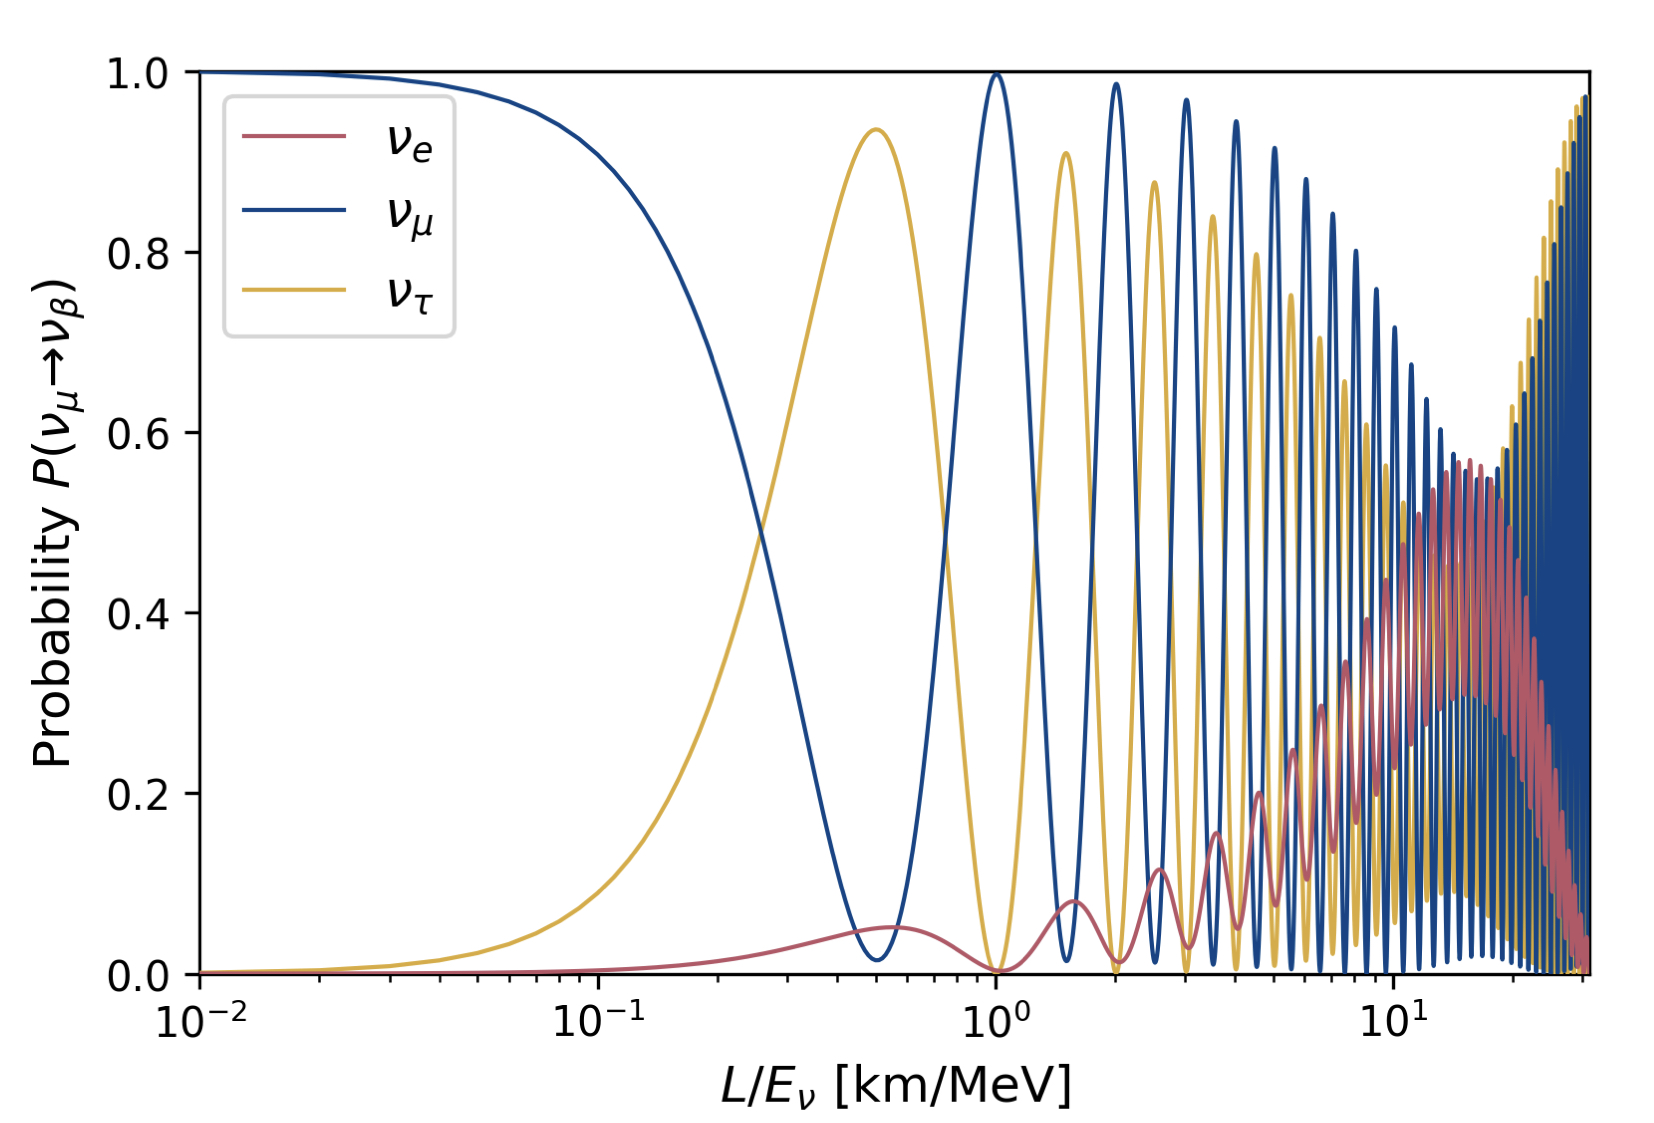
\includegraphics[scale=0.2]{Figures/three_flavor_osc.jpg}
		\caption[Three Flavor Oscillation Model]{\textbf{Three Flavor Oscillation Probabilities as a Function of L/E$_{\nu}$} \\Three Flavor Oscillation Probabilities as a Function of L/E$_{\nu}$, assuming the original state is $\nu_{\mu}$, \cite{Lauren_thesis}.}
		\label{fig:nu_osc_prob}
	\end{center}
\end{figure}

For the antineutrinos, the mathematical steps are similar from the ones we just took \cite{oscillation_math}. 

\subsubsection{First Neutrino Oscillation Measurements}
The first oscillation measurements, and consequently the confirmation that neutrinos have mass, were made by the Super-Kamiokande experiment. The Super-Kamiokande detector is located 1 km underground in the Kamioka-mine, Hida-city, Gifu, Japan. It consists of a stainless-steel tank, with 39.3 m of diameter and 41.4 m tall, filled with 50,000 tons of ultra pure water. It has about of 13,000 photo-multipliers installed on the tank's wall (see image \ref{superk_picture}).
In 1998 the Super-Kamiokande collaboration published the first neutrino oscillation measurements in a paper called ``Evidence for oscillation of atmospheric neutrinos" \cite{first_kamioka_measure}.
%
\begin{figure}[h!]
	\begin{center}
		\includegraphics[scale=0.5]{Figures/superk.pdf}
		\caption[Inside Super-Kamiokande tank]{ {\textbf{Inside Super-Kamiokande tank}}\\Workers doing photomultipliers (PMTs) checking inside Super-Kamiokande detector \cite{superk_picture}.}
		\label{superk_picture}	
	\end{center}
\end{figure}
%

\section{Current Understanding of Neutrino Physics}

At this point, allow me to briefly summarize the understanding we currently have of neutrinos, obtained through the experiments and studies I mentioned above and also by many other experiments I left out from this historical overview. 

Neutrinos are chargeless leptons with small non-zero mass that only interact through the weak force. So far, we know of the existence of three types of them, that we call "flavor", and that are named after the charged lepton that accompanies them in charged-current weak interactions: electron neutrino ($\nu_e$), muon neutrino ($\nu_{\mu}$), and tau neutrino ($\nu_{\tau}$). 

The weak interaction is mediated by three bosons: The $Z^{0}$ boson, responsible for carrying the Neutral Current (NC) interactions, and the $W^{-}$ and $W^{+}$ bosons, responsible for carrying the Charged Current (CC) interactions. The Feymann Diagrams below represent said interactions. In the CC neutrino interactions, we have an incoming neutrino interacting with a nucleus' quark and producing a charged lepton, their neutrino counterpart, and a different nucleus' quark, such as to conserve charge number. In the NC the incoming and outgoing particle natures remain the same, but transfer momentum and energy. 

\begin{figure}[h!]
	\begin{center}
		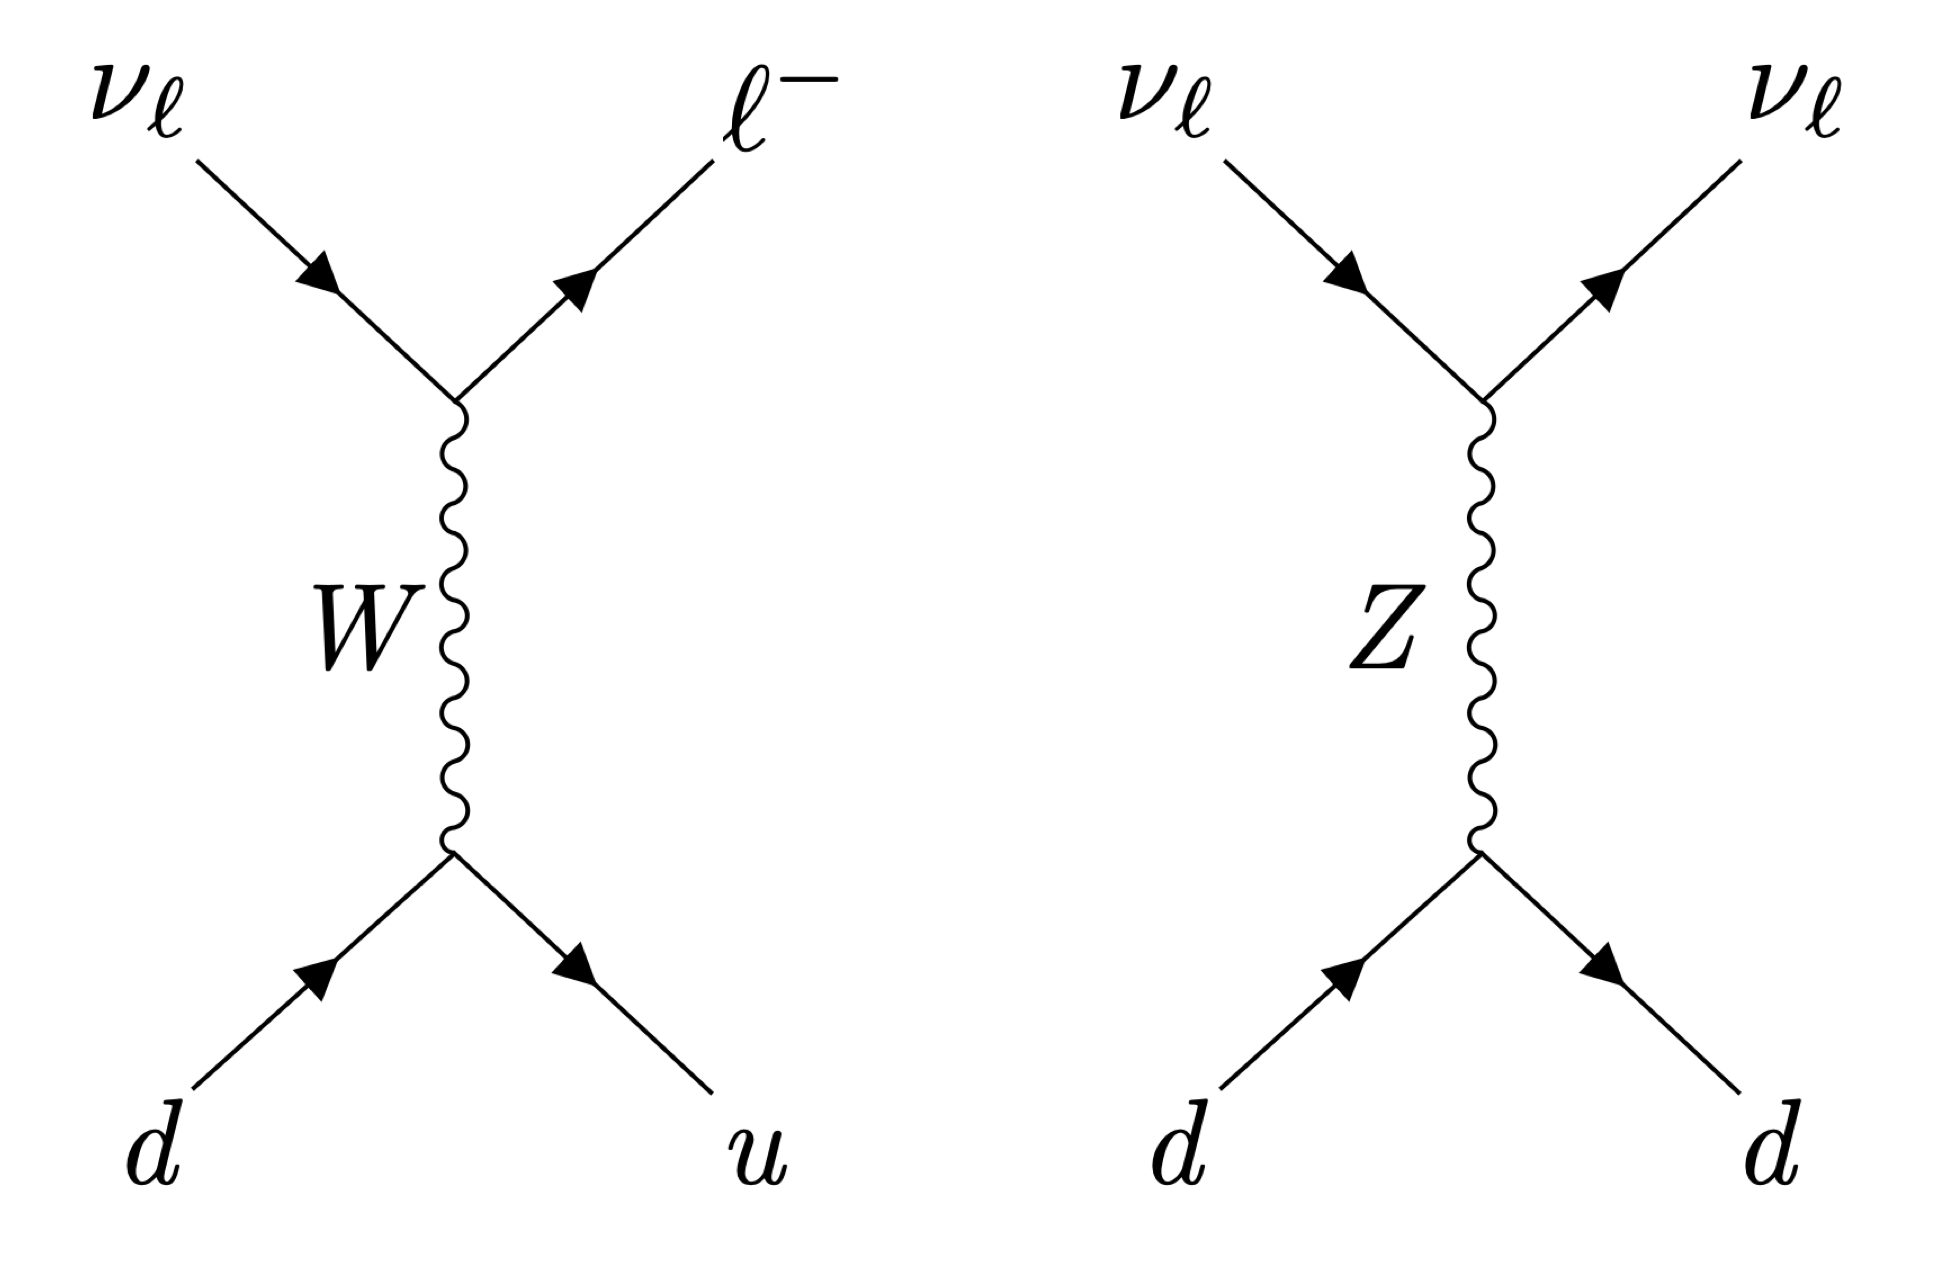
\includegraphics[scale=0.3]{Figures/feymann_diag.jpg}
		\caption[Feymann Diagrams for the two types of weak interactions]{ {\textbf{Feymann Diagrams for the two types of weak interactions}} \\ On the left, the Feymman diagram for a Charged Current interaction, carried by a W boson. On the right, the Feymman diagram for a Neutral Current interaction, carried by a Z boson, \cite{Lauren_thesis}.}
		\label{feymann_diag}	
	\end{center}
\end{figure}

We can observe different outcome final products from neutrino interactions, depending on the energy of the incoming neutrino. At lower energies, $\lessapprox 10$ GeV, the dominant processes will be quasi-elastic scattering (QE), where neutrinos scatter off of a nucleon, and resonance, where neutrinos scatter off of a nucleon that gets excited and decays. From $10$ GeV beyond, the dominant procress is Deep Inelastic Scattering (DIS) where neutrinos scatter directly off of nucleus' quarks.In figure \ref{nu_scatter} you can see a summary of the existing measurements of CC neutrino cross-section divided by neutrino energy and plotted as a function of energy. 

\begin{figure}[h!]
	\begin{center}
		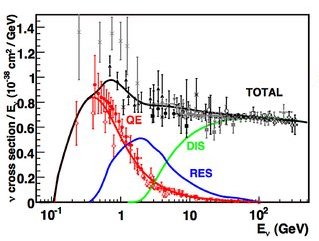
\includegraphics[scale=0.9]{Figures/nu_scatter.jpg}
		\caption[Total CC neutrino cross-section per nucleon as function of energy]{ {\textbf{Total CC neutrino cross-section per nucleon as function of energy}} \\ Summary of the existing measurements of CC neutrino-nucleon cross-section divided by neutrino energy and plotted as a function of energy. The QE is in red, the resonance in blue, the DIS in green, and the black is the total cross-section, when considering all the previous processes \cite{nu_scatter_zeller}.}
		\label{nu_scatter}	
	\end{center}
\end{figure}


%<<<<<<<<<<<<<<<<<<<<<<<<<<<<< Change Feymann Diagrams here!!! >>>>>>>>>>>>>>>>>>>>>>>>>>>>>>>>>>>>>

\subsubsection{The CP Symmetry Violating Phase Parameter}

The $\delta$ parameter showed in the PMNS matrix in equation \ref{PMNS_factored} quantifies the charge conjugation and parity symmetry violation. The strong and electromagnetic interactions are invariant under CP symmetry, but some weak interaction processes are not. This violating phase parameter is also observed in the quark sector and was already measured. The CP symmetry violating phase parameter is still not observed in the lepton sector.

\subsubsection{The Character of the Neutrino Mass Spectrum (Mass Hierarchy)}

The equation \ref{nu_oscillation_final} limits that the data of neutrino oscillation experiments can only measure the mass-squared differences. Due to the tremendous growth of the neutrino experiment efforts in the past two decades, it is known that \cite{delta_2_1}
%
\begin{equation}
	\Delta m^2_{21} = (7.53 \pm 0.18) \times 10^{-5} \ \text{eV}^2
	\label{delta_21}
\end{equation}
%
and \cite{delta_3_2}
%
\begin{equation}
	\Delta m^2_{32} = (2.34 \pm 0.09) \times 10^{-3} \ \text{eV}^2
	\label{delta_32_normal}
\end{equation}
%
or 
%
\begin{equation}
	\Delta m^2_{32} = (-2.37^{+0.07}_{-0.11}) \times 10^{-3} \ \text{eV}^2.
	\label{delta_32_inverted}
\end{equation}
%
The relative ordering $m_1 < m_2$ is known through observations of solar neutrinos, which are subject to resonant matter effects in the sun \cite{delta_2_1}. The value in \ref{delta_32_normal} corresponds to what is called Normal Hierarchy and \ref{delta_32_inverted} to what is called Inverted Hierarchy. Normal hierarchy is the condition where the $m_1 < m_2 < m_3$. Inverted hierarchy is the condition where the $m_3 < m_1 < m_2$. A schematic of the normal and inverted hierarchies can be found on figure \ref{mass_hierarchy}. The precision of neutrino sector measurements has reached a point where the unknown hierarchy is a major hurdle to further progress \cite{prospects_patterson}.

\begin{figure}
	\begin{center}
		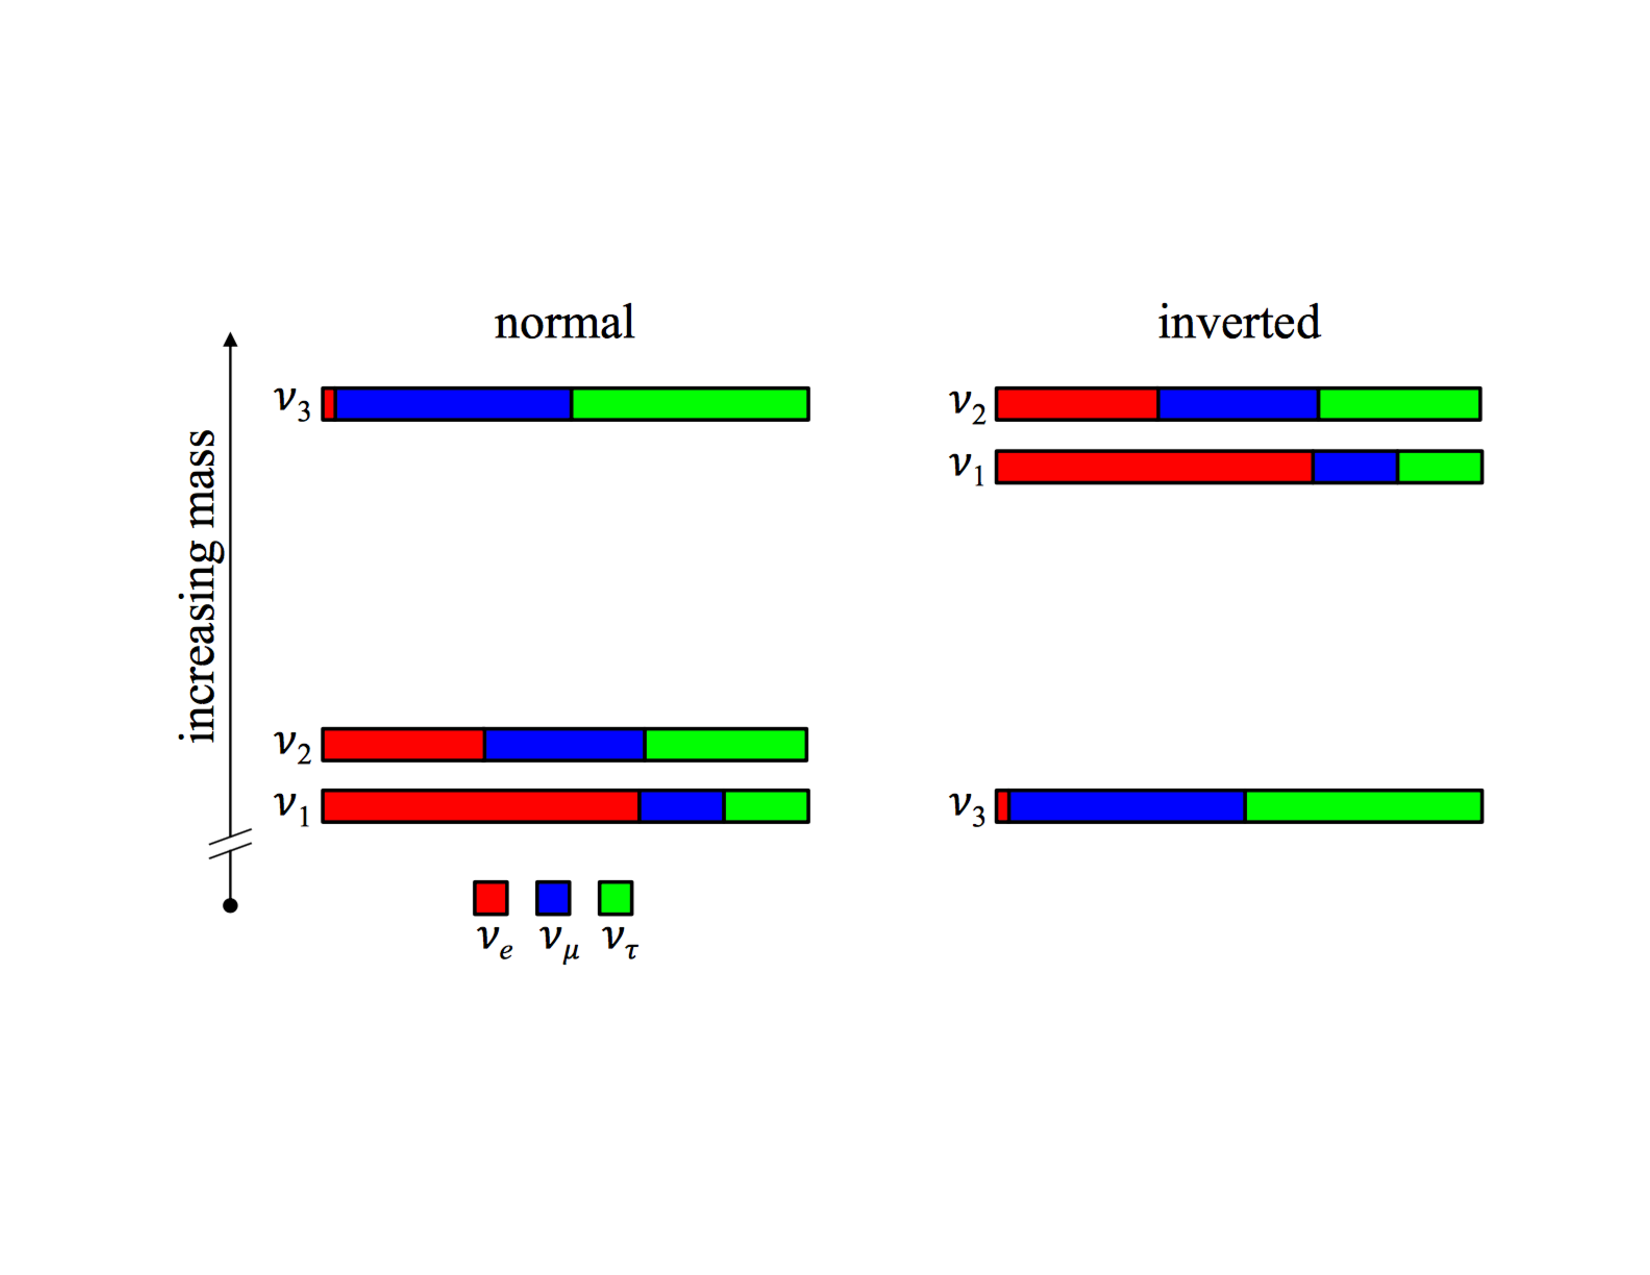
\includegraphics[scale=0.5]{Figures/mass_hierarchy.pdf}
		\caption[The Mass Hierarchy]{ {\textbf{The Mass Hierarchy}}\\The two possible neutrino mass hierarchies. The colors represent the approximate flavor admixtures present in each mass eigenstate \cite{prospects_patterson}.}
		\label{mass_hierarchy}	
	\end{center}
\end{figure}

\subsubsection{The $\mathbf{\theta_{23}}$ Octant Definition Problem}

The $\theta_{23}$ parameter is present is both $P_{\nu_\mu \rightarrow \nu_\mu}$ and $P_{\nu_\mu \rightarrow \nu_e}$ calculations. Most of the near past neutrino experiments take advantage of an approximation that considers the existence of only two neutrino flavors due to limitations in their resolution. In this approximation the oscillation probabilities take the form of
%
\begin{equation}
	P_{\nu_\mu \rightarrow \nu_e} \propto \text{sin}^2(2\theta_{23}) \ \text{ and } \ P_{\nu_\mu \rightarrow \nu_\mu} \propto \text{sin}^2(2\theta_{23}),
	\nonumber
\end{equation}
%
which implies in a redundancy in the value of $\theta_{23}$, with the possibilities being either $\theta_{23} > \pi/4$ or $\theta_{23} < \pi/4$. 
In more recent results, experiments such as NuMI Off-axis $\nu_e$ Appearance (NO$\nu$A), Main Injector Neutrino Oscillation (MINOS) and Tokai to Kamioka (T2K), do not use this approximation, resulting in a 2 fold degeneracy solution for the mixing angle $\theta_{23}$. The latest results were presented by the NO$\nu$A Collaboration and can be seen in figure \ref{nova_result}, which shows the two best fit values with their 90\% confidence level contours. In this study, NO$\nu$A Collaboration disfavored the maximal mixing ($sin^2 \theta_{23} = 0.5$) scenario with $2.6 \sigma$ significance \cite{NOVA}.

\begin{figure}
	\begin{center}
		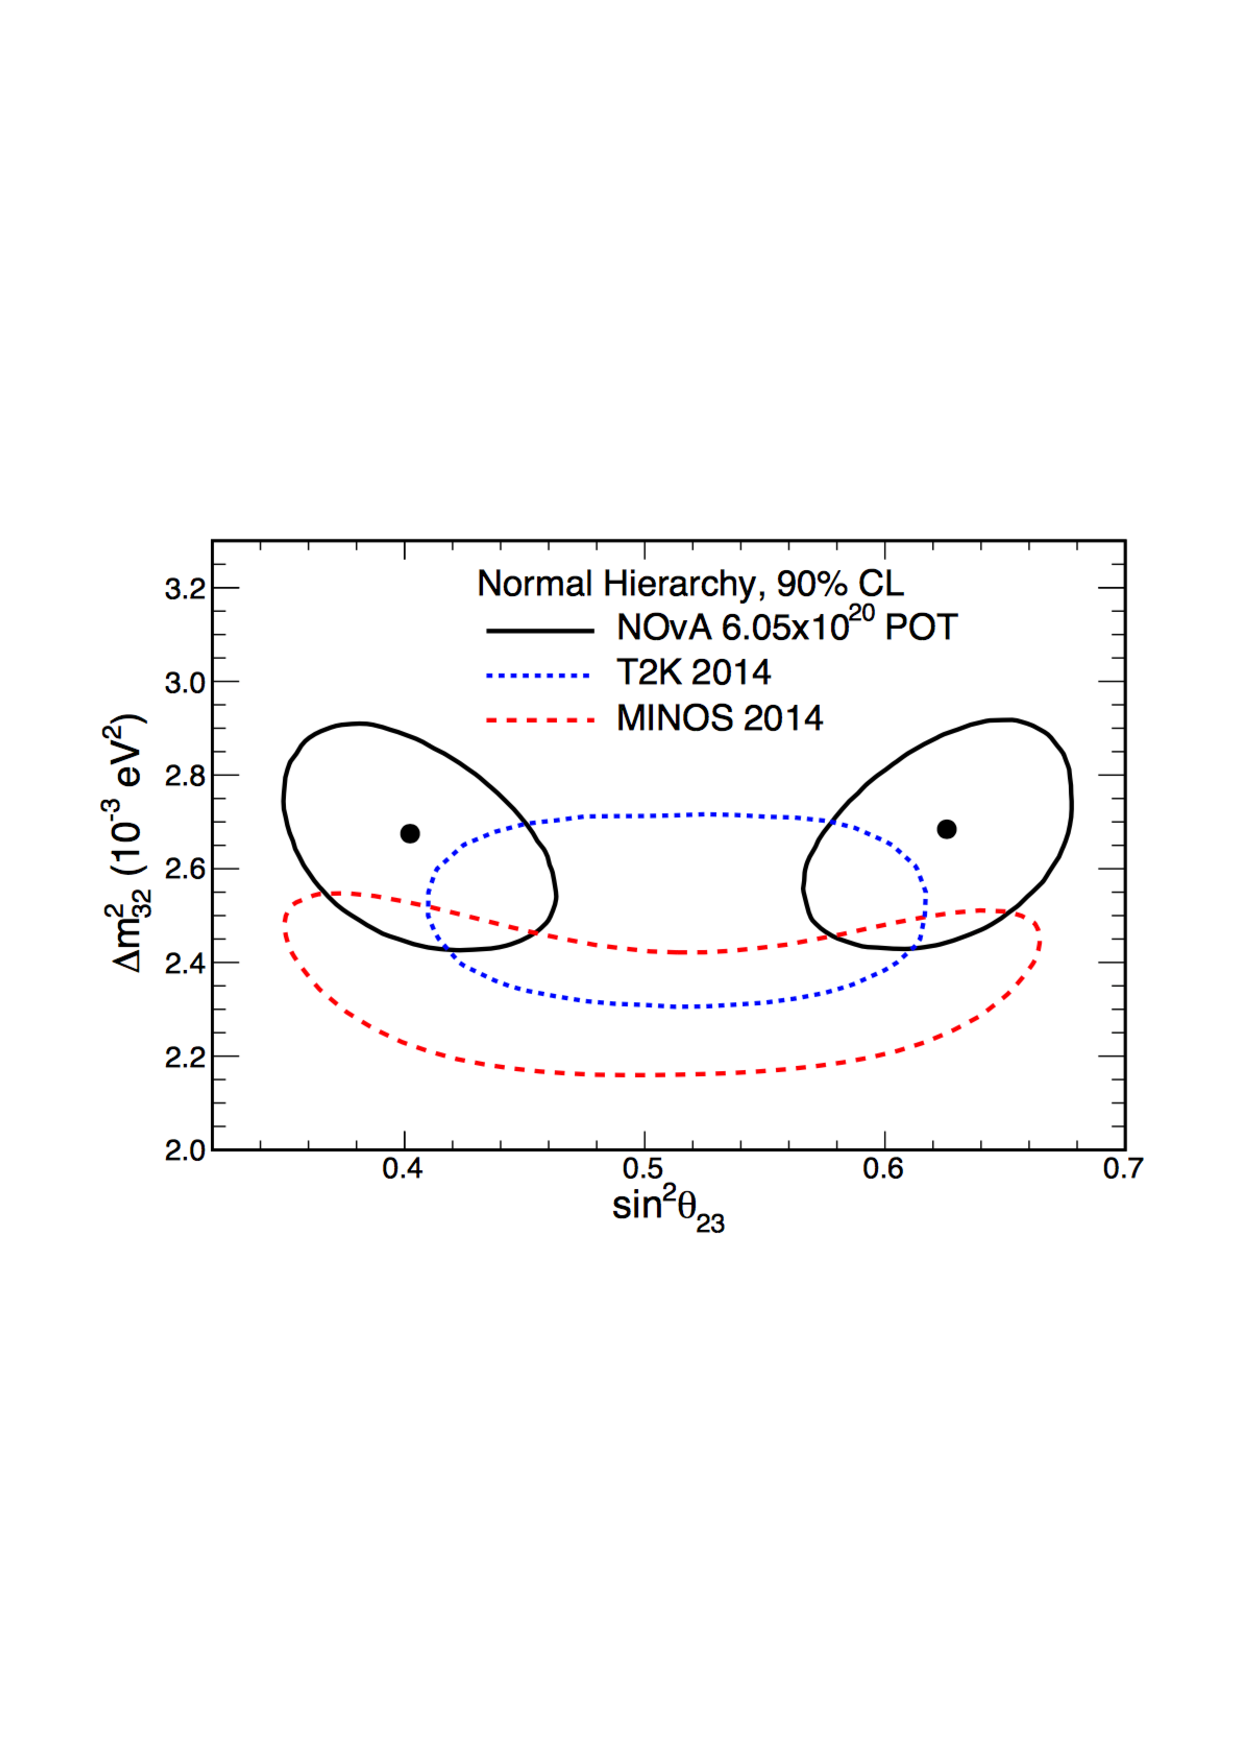
\includegraphics[scale=0.7]{Figures/nova_result.pdf}
		\caption[Preliminary $\theta_{23}$ results from the NO$\nu$A Experiment]{ {\textbf{Preliminary $\theta_{23}$ results from the NO$\nu$A Experiment}} \\ Best fit (black dots) and allowed $90\%$ confidence level regions (solid black curves) of $\sin^2 \theta_{23}$ and $\Delta m^2_{23}$ for the normal hierarchy. The dashed curves show MINOS \cite{MINOS} and T2K \cite{T2K} $90\%$ confidence level contours \cite{NOVA}.}
		\label{nova_result}	
	\end{center}
\end{figure} 


\subsubsection{Low Energy Excess (LEE) Anomalies}

Over the past few decades, a number of neutrino experiments found inconsistencies between their expected un-oscillated neutrino flux at low energies and their measurements. Allow me to describe a few of them briefly. The Liquid Scintillator Neutrino Detector (LSND) at the Los Alamos Neutron Science Center published a paper in 2001 where they had found an excess of electron-like antineutrino events in a primarily $\nu_{\mu}$ beam \cite{lsnd}. Years later, the MiniBooNE Experiment probed the same $L/E_{\nu}$ region and also found an excess of electron-like neutrino and antineutrino events in a primarily $\nu_{\mu}$ and $\bar{\nu_{\mu}}$ respectively, depending of the polarity of the Booster Neutrino Beam (BNB). Due to limitations on MiniBooNE's detector technology to separate electron and photon showers, their analysis was inconclusive as to whether the excess was due to new physics or due to background mis-modeling, \cite{miniboone}. To address this issue, a new detector with better technology for particle identification was placed near MiniBooNE. This new experiment, named MicroBooNE, published its results recently, in 2021. In this new report, they did not find an excess of electron-like neutrino events, but could not refute MiniBooNE's excess either \cite{microboone_lee}. The favorite hypothesis for new physics that could explain the LEE phenomena is that there would exist a fourth neutrino, called sterile neutrino $\nu_s$. This neutrino, unlike the others, would only interact through the weak force and therefore would only be indirectly observed whenever oscillating from or to one of the other flavors, which would justify the LEE observed, \cite{Lauren_thesis}. 
The LEE Anomaly and the of $\nu_s$s remain open questions in the field. 

\section{LArTPCs in Neutrino Physics}

Among a wide variety of detector technologies, Liquid Argon Time Projection Chambers (LArTPCs) present a set of characteristics particularly interesting to neutrino physics. 
In a more general form, Time Projection Chambers were first proposed by David Nygren, in 1974 \cite{Nygren} and they consist of a volume filled with a sensitive gas or liquid in a strong ($\sim$500 V/cm) electrical field. When a charged particle passes through the active volume of the detector, the material is ionized, leaving behind a track of ionization charge. This ionization charge is then drifted by an electrical field towards wire planes, where sensitive electronics will record the induction signal, from the passing electrons throught the wires, and current, produced by the collection of the electrons by the last set of wires (see figure \ref{lartpc}). Using a two (or more) plane setup, with at least one being an induction plane and the other being a collection plane, and a light trigger to calculate the drift time of the electrons in the event, it is possible to have a three dimensional calorimetric reconstruction of the track (see figure \ref{lartpc_readout}).

\begin{figure}[h!]
	\begin{center}
		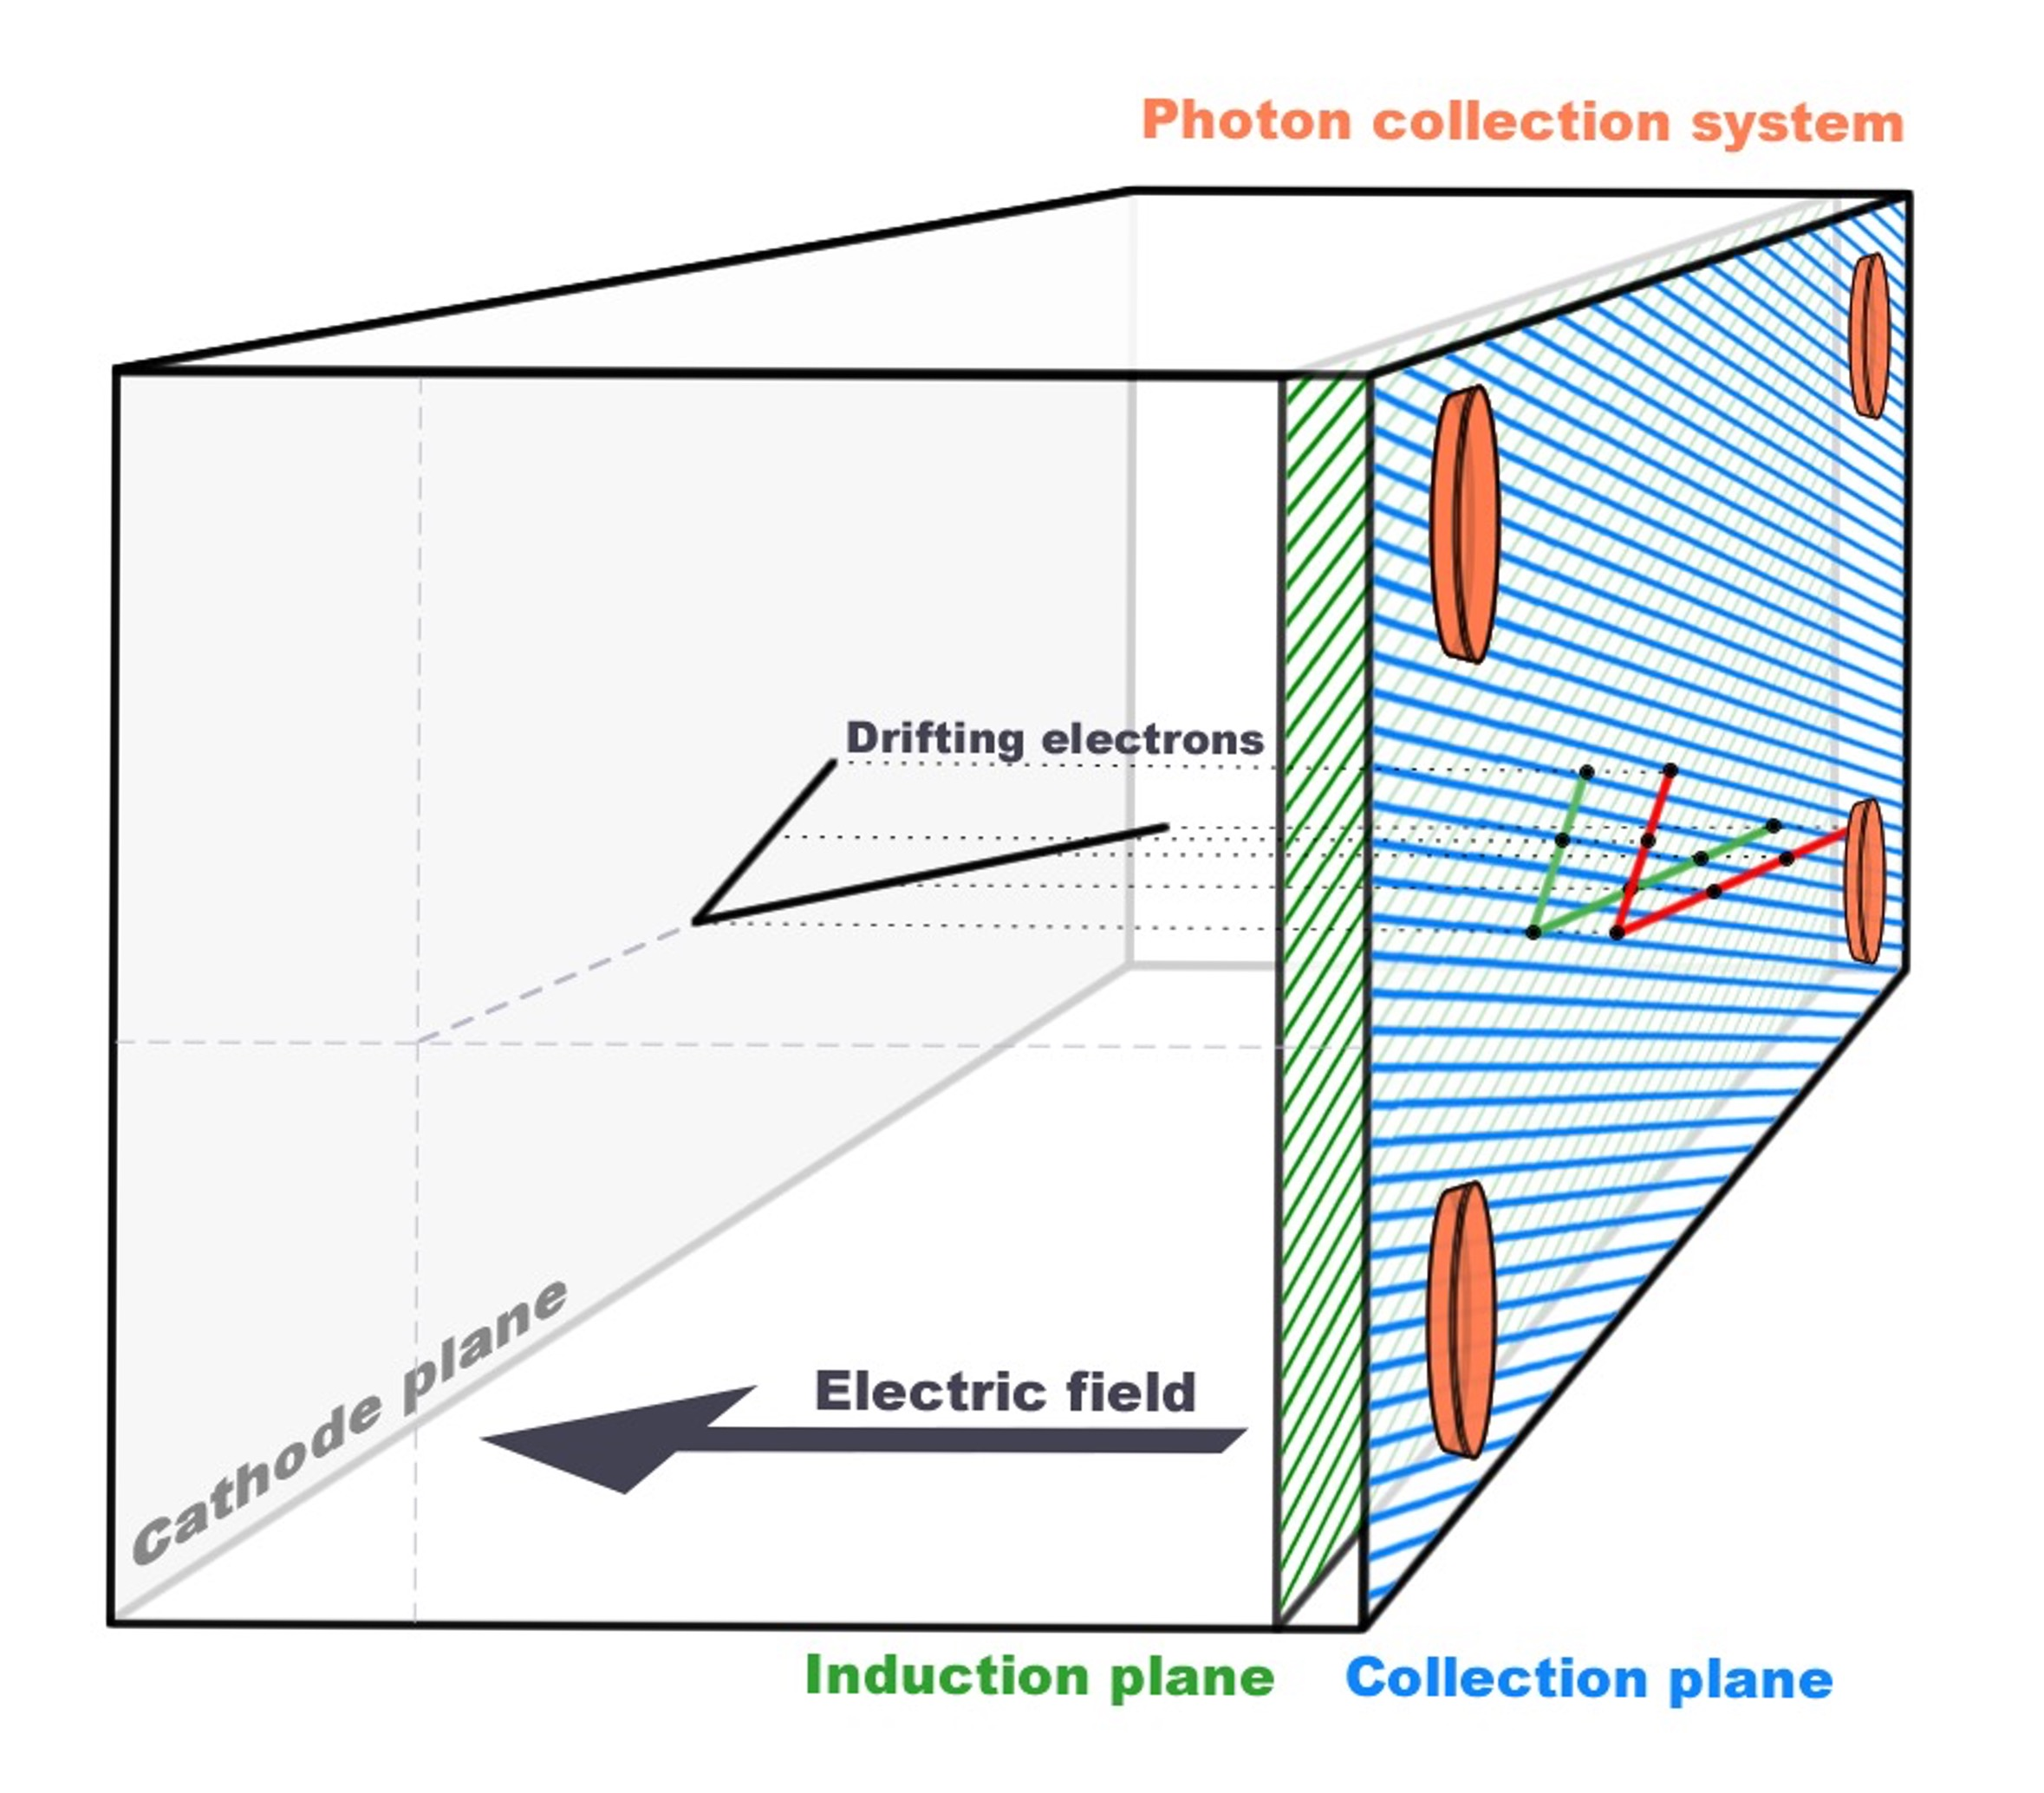
\includegraphics[scale=0.1]{Figures/LARTPC.jpg}
		\caption[LArTPC]{ {\textbf{Liquid Argon Time Projection Chamber}} \\ Liquid Argon Time Projection Chamber. When a particle passes through its fiducial volume and interacts with the liquid argon, ionization electrons and scintillation light are produced. The electric field drifts the electrons from where they are produced towards the planes of wires (right corner in the figure). Both charge and light produced are read by precision wires and a light collection system (in the figure, the orange bodies behind the wires), respectively.}
		\label{lartpc}	
	\end{center}
\end{figure}

\begin{figure}
	\begin{center}
		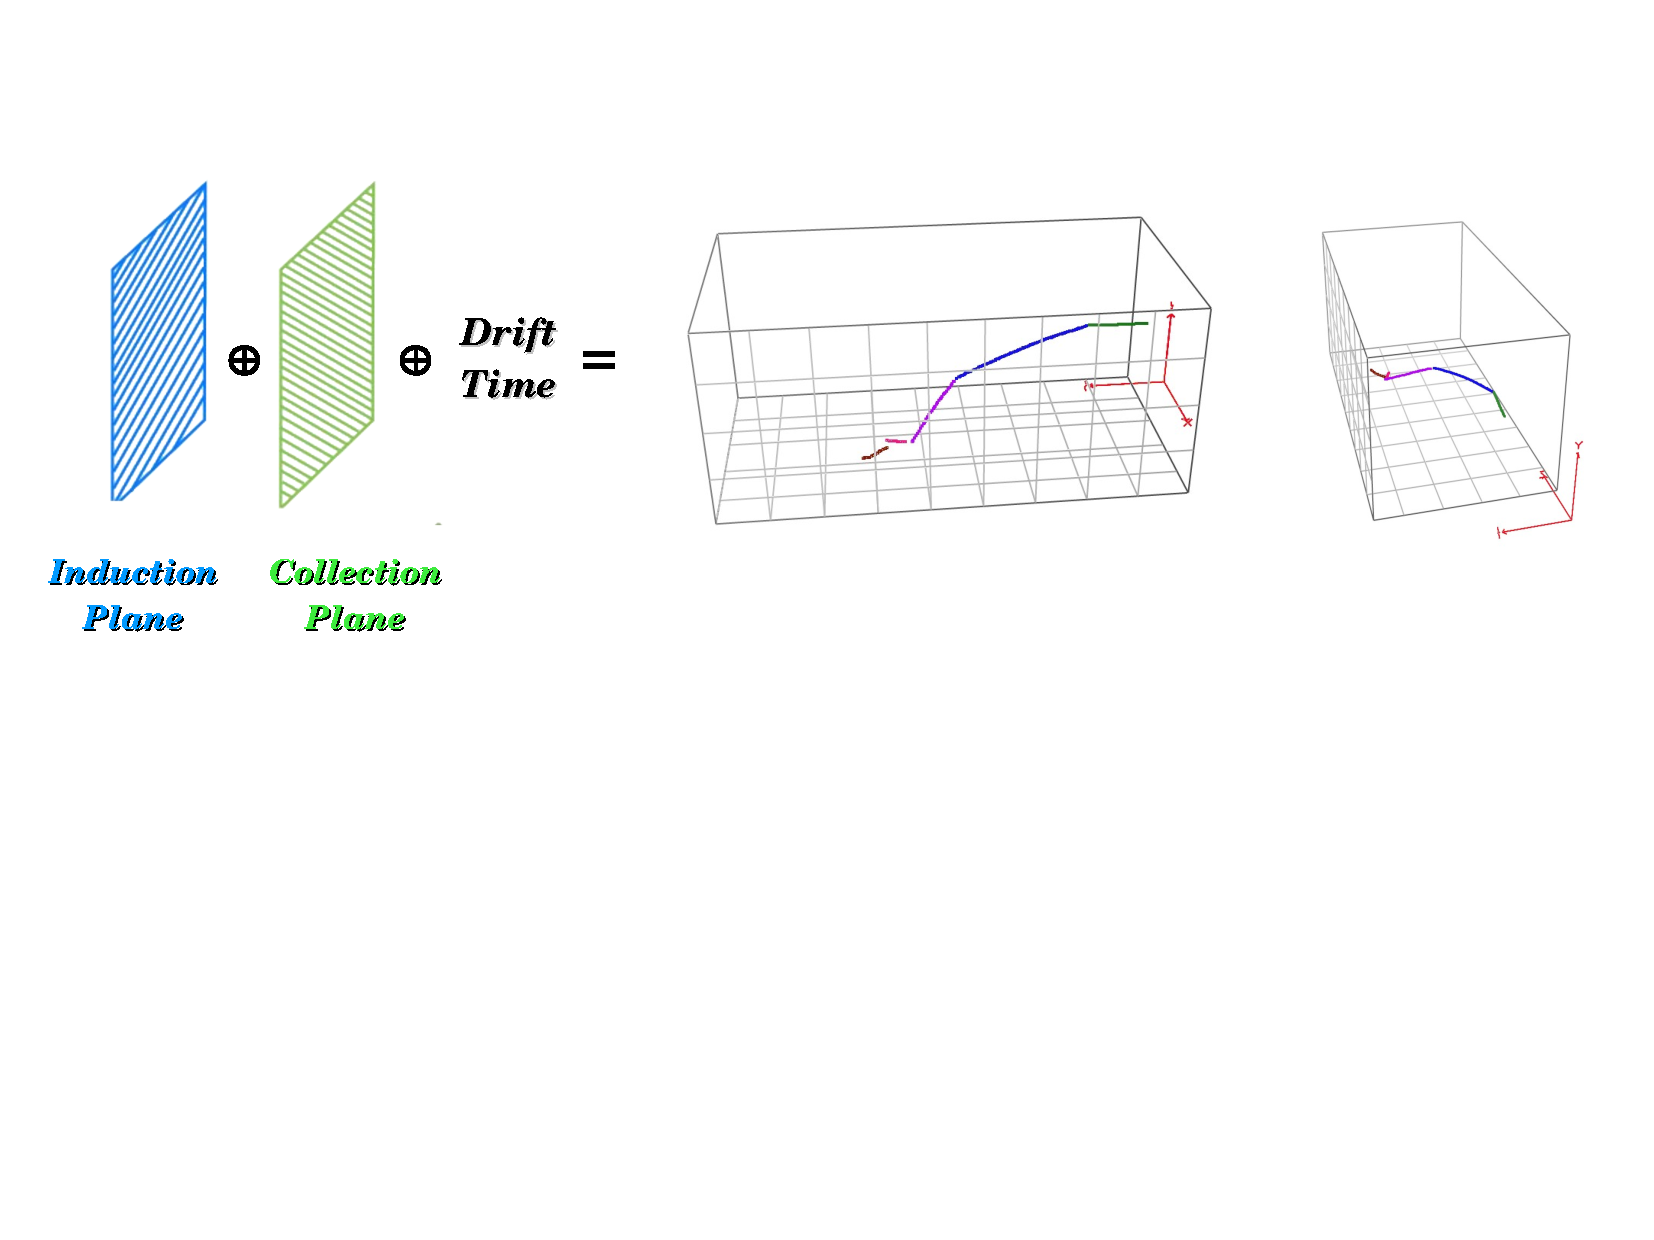
\includegraphics[scale=0.6]{Figures/Acciarri_fig2.pdf}
		\caption[LArTPC read out system]{ {\textbf{LArTPC read out system}} \\ Basic elements of the LArTPC read out system. It is needed a minimum of one induction wire plane, one collection wire plane and a light detection system. The information retrieved by those 3 components allow a 3D track reconstruction \cite{Acciarri_presentation}.}
		\label{lartpc_readout}	
	\end{center}
\end{figure}

\newpage
Not long after, in 1977, Carlo Rubia noted that using Liquid Argon (LAr) as active material in a TPC was particularly advantageous for neutrino physics, since:
\begin{itemize}
	\item it is dense (1.4 g/cm$^3$), which increases the interaction probability;
 	\item it does not attach electrons, allowing long drift distances, which allows the construction of big detectors;
  	\item it has a high electron mobility;
   	\item argon is the third most abundant gas in the atmosphere, it is easy to obtain and purify, making it relatively cheap;
  	\item it is inert and and can be liquified with liquid nitrogen \cite{Rubia_ANewConcept}
\end{itemize}

Ever since, LArTPCs have been the technology of choice of many neutrino physics experiments, such as  Imaging Cosmic and Rare Underground Signals (ICARUS), \cite{ICARUS_proposal}, MicroBooNE, \cite{microboone_proposal}, Short Baseline Neutrino Detector (SBND), \cite{SBND}, that together form the Short Baseline Neutrino (SBN) Program, and Deep Underground Neutrino Experiment (DUNE) \cite{dune_snowmass_22}, to name a few. 

\section{The Short Baseline Neutrino Program}

In a new attempt to get to a conclusion regarding the LEE, described in session, Fermilab created the SBN Program. The program consists of three LArTPCs (SBND, MicroBooNE, and ICARUS) all located along the BNB beam. The principle is that, by having three different detectors of the same technology, exposed to the same beam, and all positioned at a short-baseline range, we will be more accurately be able to constrain our flux of neutrinos and possibly have an answer to the LEE anomalies observed so far, and search for sterile neutrinos. Beyond that, it aims to study neutrino-nucleus scattering at the GeV energy scale and further develop LArTPC's construction and installation procedures, \cite{SBN}.

Originally, ICARUS was, the first large-scale LArTPC to be used to further our understanding of neutrinos and was located underground at the The Gran Sasso National Laboratory and exposed to the CERN Neutrinos to Gran Sasso (CNGS) beamline \cite{ICARUS_proposal}. Most recently one of its modules, the T600, was refurbished, upgraded and has its new home at Fermilab, in the BNB beam. ICARUS T600 LArTPC is used as the far detector in the SBN Program. It is a $476$ton active mass LArTPC and it seats $600$ m from the target. 

\begin{figure}[h!]
	\begin{center}
		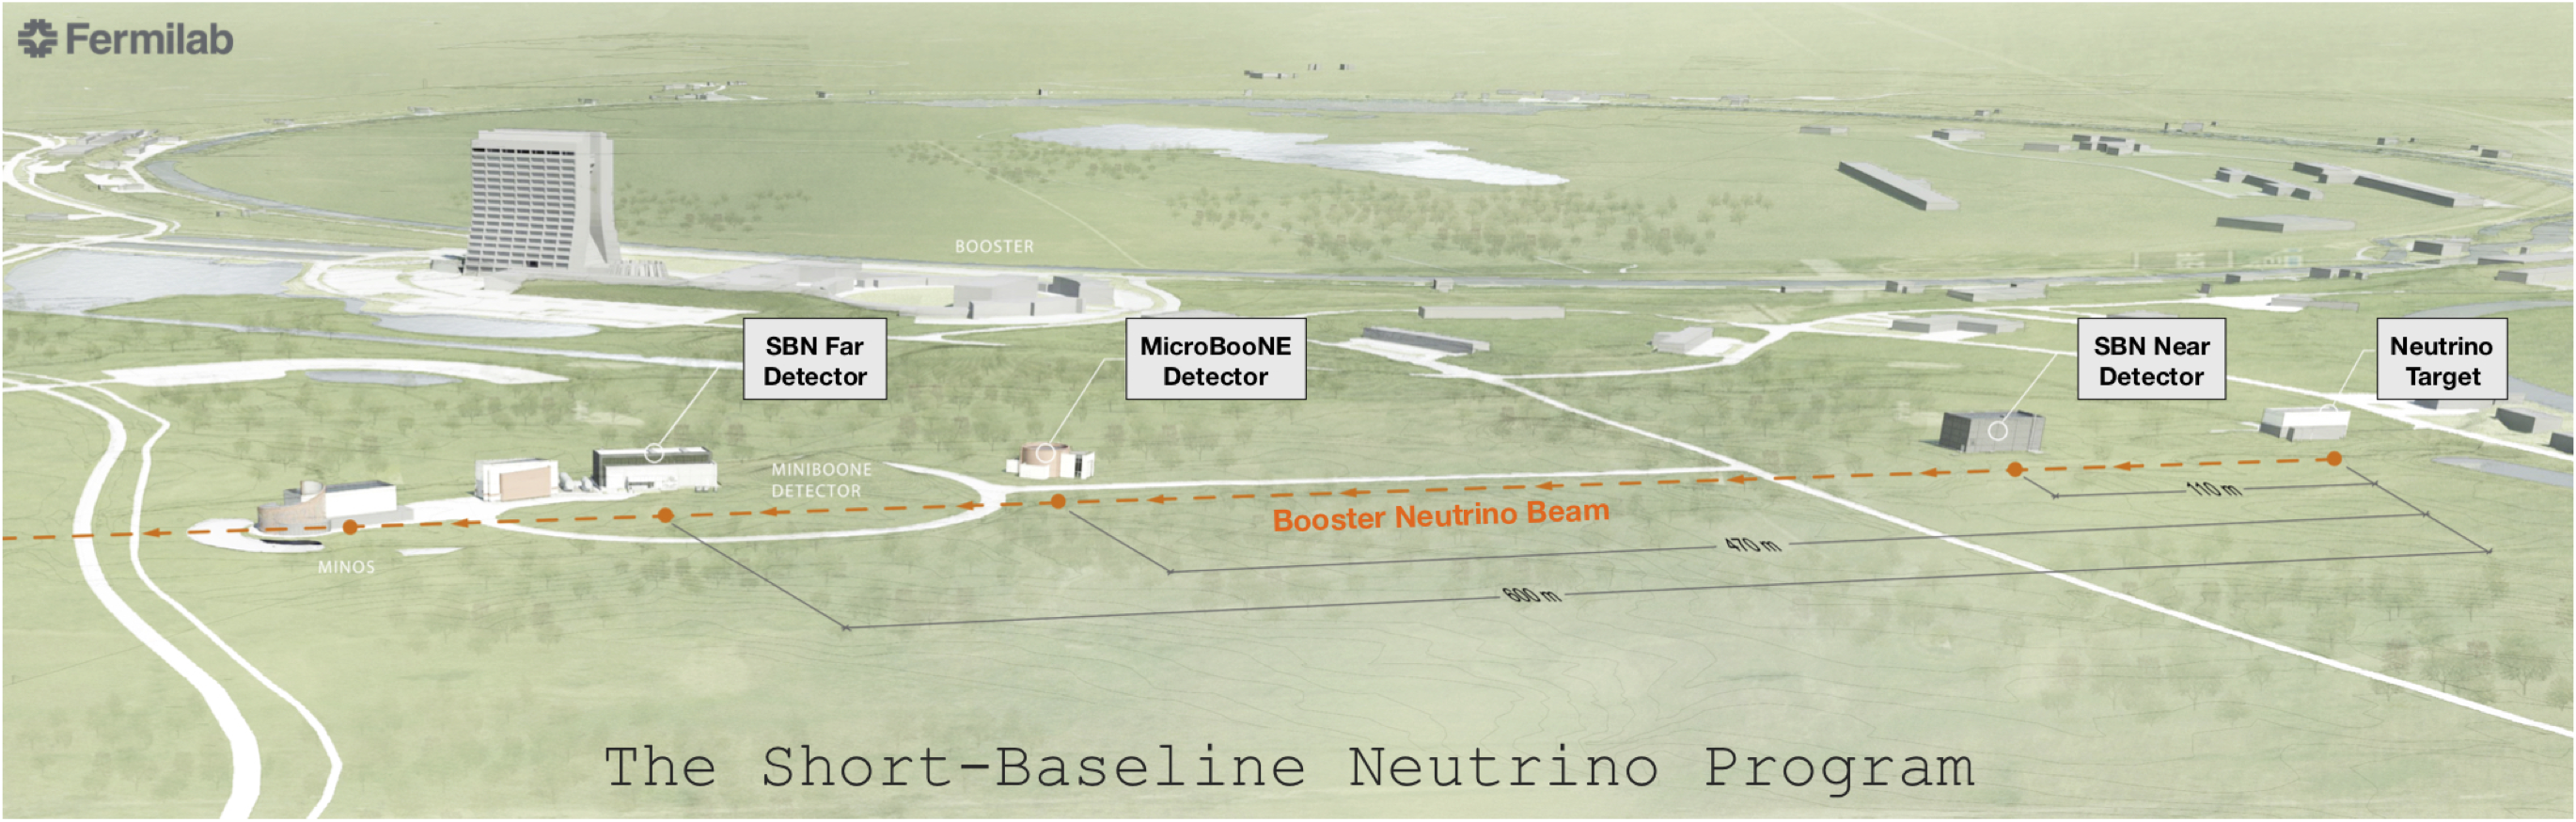
\includegraphics[scale=0.32]{Figures/SBN.png}
		\caption[The Short-Baseline Neutrino Program]{\textbf{The Short-Baseline Neutrino Program}\\The Short-Baseline Neutrino Program detectors as seen from an upper view at Fermilab. To the right is the neutrino beam target area where $8$ GeV protons from the Booster accelerator impinge a beryllium target. The beam is focused along the orange dashed line traveling toward the left (north). The SBND, MicroBooNE, and ICARUS, \cite{SBN}.
		}
		\label{sbn_program}
	\end{center}
\end{figure}

The SBND is, as the name implies, the program's near detector and it consists of a $112$ton active mass LArTPC is at $110$ m from the target. It is currently under  installation phase and it is expected to be taking date mid-late next year,2023. In-between ICARUS and SBND, at $470$ m from the target, there is MicroBooNE, a $89$ton active volume LArTPC that has been taking da since 2015. Where each of the detectors are in the BNB beamline, at Fermilab, is illustrated in figure \ref{sbn_program}.
I will later describe in more details SBND and MicroBooNE, as they are the experiments in which I've carried my Ph.D. work. 

\section{The Deep Underground Neutrino Experiment}

The Deep Underground Neutrino Experiment (DUNE) is by far the most promising experiment for neutrino physics, as it aims to measure the CP violating phase in the leptonic sector, to determine the character of the neutrino mass spectrum, and to make precision measurements of oscillation parameters. Beyond the neutrino physics goals, DUNE also aims to search for baryon number violating processes and to perform precision measurements of neutrinos from a core-collapse supernova within the Galaxy, if one happens during the experiment's operating period. 
To accomplish such bold goals, DUNE counts with a near detector placed at Fermilab and a far detector at the Sanford Underground Research Laboratory in Lead, South Dakota. An intense neutrino beam of up to $2.4$ megawatts is produced at Fermilab, crosses the near detector, and travels $1,300$ kilometers downstream through Earth's crust to reach the far detector. In figure \ref{DUNE_full_schematic} you can see an schematic diagram of the experiment. 

\begin{figure}[h!]
	\begin{center}
		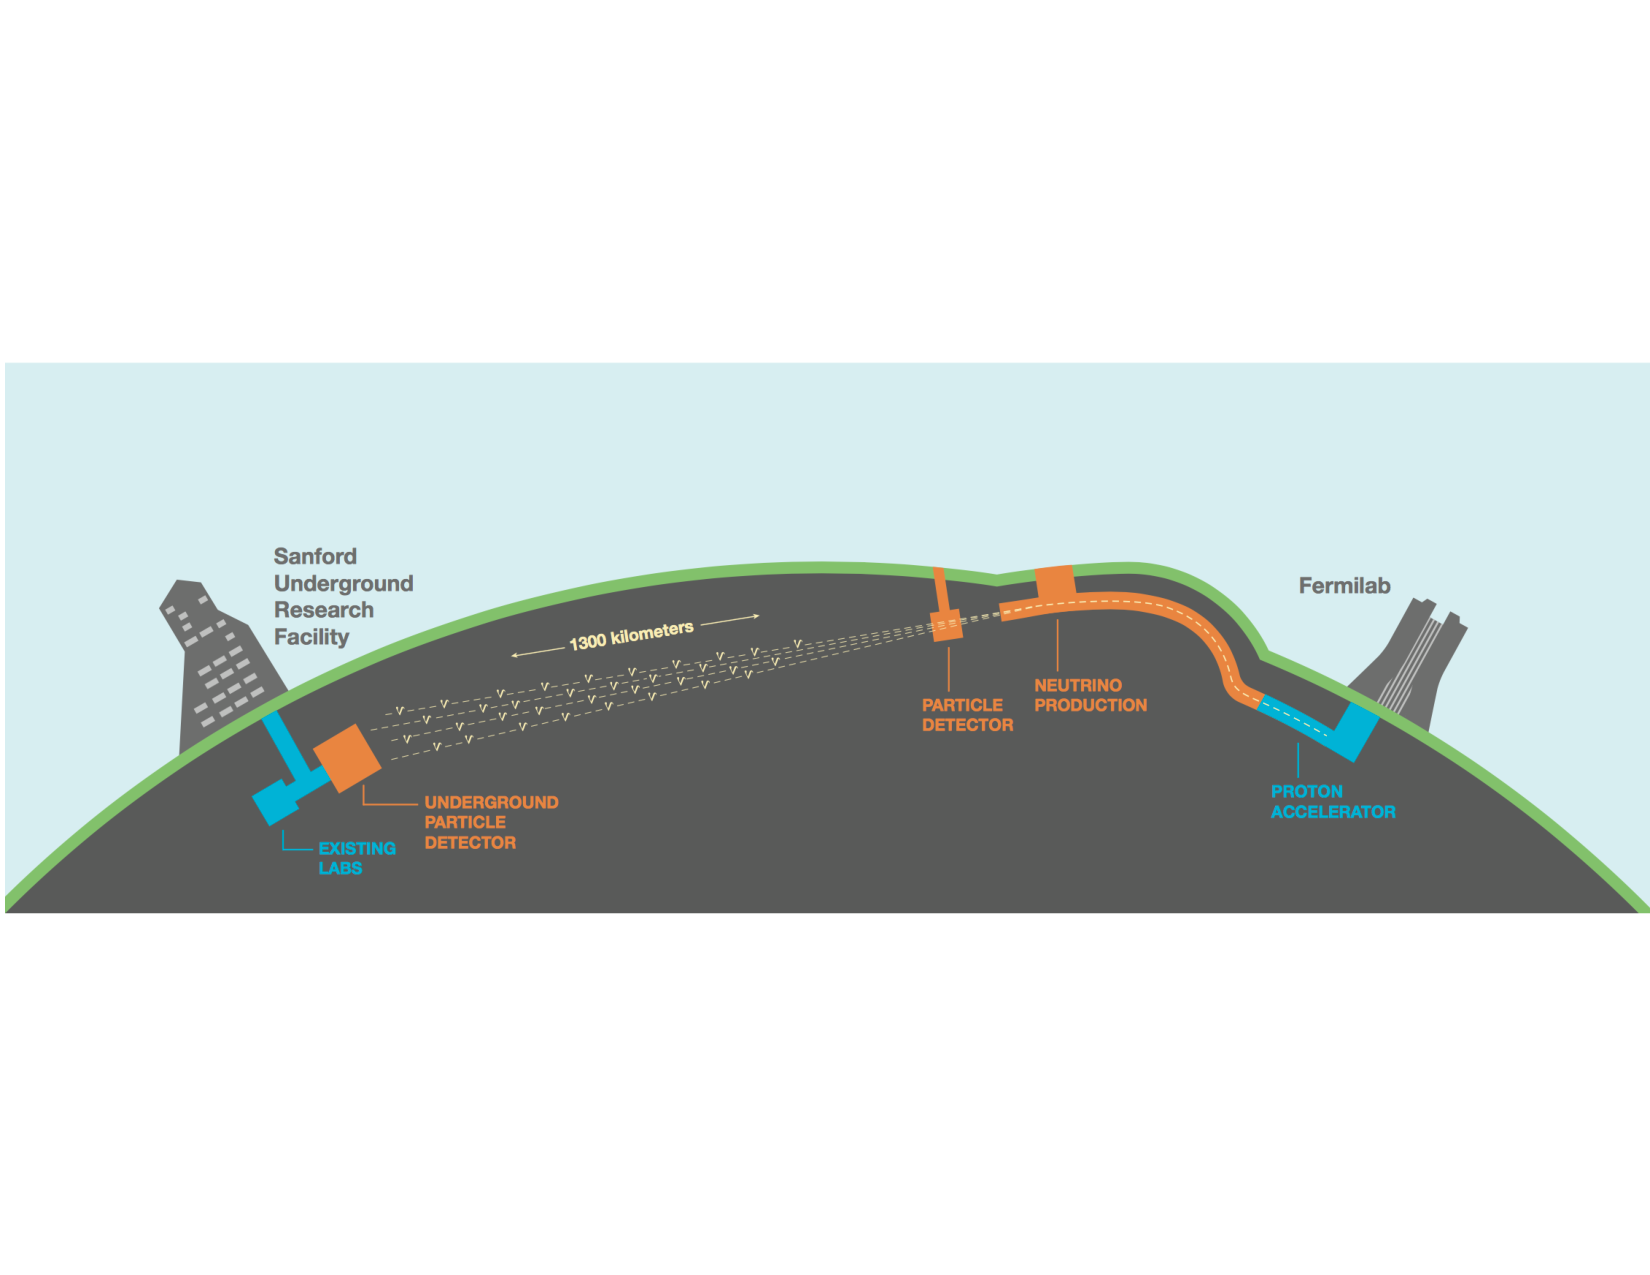
\includegraphics[scale=0.6]{Figures/DUNE_full_schematic.pdf}
		\caption[DUNE's full schematic]{ {\textbf{DUNE's full schematic.}} \\The figure shows the full DUNE's schematics, providing a view of the production of the neutrino beam, the Near Detector at Fermilab, the under crust travel of the beam, and the Far Detector at SURF, \cite{dune_snowmass_22}.}
		\label{DUNE_full_schematic}	
	\end{center}
\end{figure}

DUNE's far detector is made of $4$ LArTPCs modules, of $10$ kton each. The near detector will have a combination of three different detection systems: a modular and optically segmented LArTPC of $\approx300$ tons (ND-LAr), a magnetized high-pressure Gas Argon Time Projection Chamber (GArTPC) surrounded by a calorimeterm (ND-GAr), a magnetized beam monitor consisting of an electromagnetic calorimeter, an inner target/tracker system and an active LAr target (SAND). \cite{dune_snowmass_22, dune_SAND}.